%\documentclass[tikz, border=5pt]{standalone}
\begin{document}
	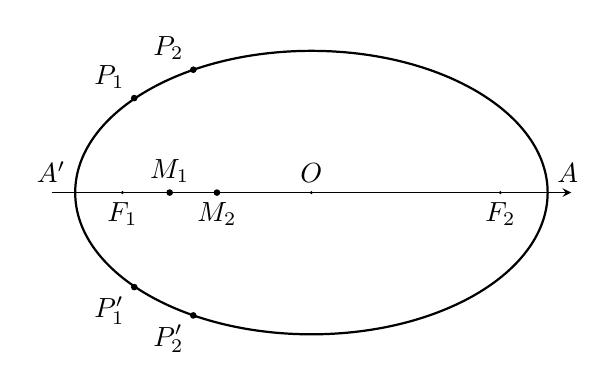
\begin{tikzpicture}[>=stealth, scale=0.6]
		% 1. 定义椭圆参数(长半轴a=5,短半轴b=3,焦距c=4)
		\def\a{5}  % 长半轴
		\def\b{3}  % 短半轴
		\def\c{4}  % 焦距(c = sqrt(a² - b²) = 4)
		
		% 2. 绘制椭圆
		\draw[thick] (0,0) ellipse ({\a} and {\b});
		
		% 3. 绘制x轴(含标记点)
		\draw[->] (-5.5,0) -- (5.5,0);
		\fill (-5,0) circle (1pt) node[above left] {$A'$};  % 左顶点
		\fill (5,0) circle (1pt) node[above right] {$A$};   % 右顶点
		\fill (0,0) circle (1pt) node[above] {$O$};   % 原点O
		\fill (-4,0) circle (1pt) node[below] {$F_1$}; % 左焦点
		\fill (4,0) circle (1pt) node[below] {$F_2$}; % 右焦点
		
		% 4. 标记线段上的点 M1, M2
		\coordinate (M1) at (-3, 0); % 点 M1
		\coordinate (M2) at (-2, 0);   % 点 M2
		\fill (M1) circle (2pt) node[above] {$M_1$};
		\fill (M2) circle (2pt) node[below] {$M_2$};
		
		% 6. 绘制圆弧
%		\draw (-4,0) circle (2) ;
%		\draw (-4,0) circle (3) ;
		
		% 5. 标记椭圆上的点 P1, P2, P'1, P'2
		\coordinate (P1) at (-3.75, 2);   % 上半部分点 P1
		\coordinate (P2) at (-2.5, 2.6);   % 上半部分点 P2
		\coordinate (P1p) at (-3.75, -2); % 下半部分点 P'1
		\coordinate (P2p) at (-2.5, -2.6); % 下半部分点 P'2
		\fill (P1) circle (2pt) node[above left] {$P_1$};
		\fill (P2) circle (2pt) node[above left] {$P_2$};
		\fill (P1p) circle (2pt) node[below left] {$P'_1$};
		\fill (P2p) circle (2pt) node[below left] {$P'_2$};
		
	\end{tikzpicture}
\end{document}
